\documentclass[a4paper,11pt]{article}
%%\documentclass[a4paper,12pt]{amsart}
\usepackage[cp1252]{inputenc}
\usepackage[spanish]{babel}
\usepackage{amsmath}
\usepackage{amsthm}
\usepackage{amssymb}
\usepackage{amsfonts}
\usepackage{graphicx}
\usepackage{cancel}
\usepackage{color}
\usepackage{multirow}
\usepackage{colortbl}

\setlength{\textheight}{23.5cm} \setlength{\evensidemargin}{0cm}
\setlength{\oddsidemargin}{-0.8cm} \setlength{\topmargin}{-2.5cm}
\setlength{\textwidth}{17.5cm} \setlength{\parskip}{0.25cm}

\hyphenation{pro-ba-bi-li-dad}
\spanishdecimal{.}

\newtheoremstyle{teoremas}{\topsep}{\topsep}%
     {}% Body font
     {}% Indent amount (empty = no indent, \parindent = para indent)
     {}% Thm head font
     {}% Punctuation after thm head
     {0.5em}% Space after thm head (\newline = linebreak)
     {\thmname{{\bfseries#1}}\thmnumber{ {\bfseries#2}.}\thmnote{ {\itshape#3}.}}% Thm head spec
\theoremstyle{teoremas}

\newtheorem{teorema}{Teorema}[section]
\newtheorem{corolario}[teorema]{Corolario}


\newtheoremstyle{ejemplos}{\topsep}{\topsep}%
     {}%         Body font
     {}%         Indent amount (empty = no indent, \parindent = para indent)
     {}%         Thm head font
     {.}%        Punctuation after thm head
     {0.5em}%     Space after thm head (\newline = linebreak)
     {\thmname{{\bfseries#1}}\thmnumber{ {\bfseries#2}}\thmnote{ {\itshape#3}}}%         Thm head spec
\theoremstyle{ejemplos}

\newtheoremstyle{definiciones}{\topsep}{\topsep}%
     {}%         Body font
     {}%         Indent amount (empty = no indent, \parindent = para indent)
     {}%         Thm head font
     {.}%        Punctuation after thm head
     {0.5em}%     Space after thm head (\newline = linebreak)
     {\thmname{{\bfseries#1}}\thmnumber{ {\bfseries#2}}\thmnote{ {\itshape#3}}}%         Thm head spec
\theoremstyle{definiciones}

\newtheoremstyle{lemas}{\topsep}{\topsep}%
     {}%         Body font
     {}%         Indent amount (empty = no indent, \parindent = para indent)
     {}%         Thm head font
     {.}%        Punctuation after thm head
     {0.5em}%     Space after thm head (\newline = linebreak)
     {\thmname{{\bfseries#1}}\thmnumber{ {\bfseries#2}}\thmnote{ {\itshape#3}}}%         Thm head spec
\theoremstyle{lemas}


\newtheorem*{definicion}{Definici\'on}
\newtheorem*{enunciado}{Enunciado}
\newtheorem*{solucion}{Soluci\'on}
\newtheorem*{demostracion}{Demostraci\'on}
\newtheorem*{lema}{Lema}
\newtheorem*{hipotesis}{Hip\'otesis}
\newtheorem*{estadistico}{Estad\'{\i}stico de Prueba}
\newtheorem*{region}{Regi\'on de Rechazo}
\newtheorem*{conclusion}{Conclusi\'on}
\newtheorem*{hallar}{Por hallar}
\newtheorem*{observaciones}{Observaciones}
\newtheorem*{propiedades}{Propiedades}


\title{Notas sobre el origen del angulo entre vectores abstractos}
\author{\'Alvaro J. Carde\~na Mej\'{\i}a}
\date{\today}

\begin{document}

\maketitle

\section{Motivaci\'on}

En el libro \textit{\'Algebra Lineal y Geometr\'{\i}a Cartesiana}, de Juan de Burgos (2a ed.), se menciona que hay un an\'alisis que detalla el concepto de \'angulo entre vectores definido con exactitud; sin embargo, el autor considera dif\'{\i}cil y que no se han precisado conceptos hasta el momento en que inicia aquella discusi\'on. De este modo, el autor hace referencia a un ap\'endice del libro para quien desee entender a detalle el origen del concepto y comienza el apartado usando la caracterizaci\'on de un \'angulo entre vectores a partir de su coseno, dejando lagunas l\'ogicas en la construcci\'on de los conceptos.
\par 
A pesar de todo, el mencionado ap\'endice no se encuentra en el libro y no parece que haya en el mismo una construcci\'on o an\'alisis detallado sobre el concepto a tratar.
\par
De este modo, me propuse buscar una construcci\'on rigurosa del concepto en s\'{\i} sin mucho \'exito, ya que muchos libros de \'algebra lineal tienden a iniciar la discusi\'on con la misma caracterizaci\'on del coseno del \'angulo y otras m\'as siguen conteniendo lagunas l\'ogicas.
\par 
Es por ello que decid\'{\i} contruir por mi propia cuenta el an\'alisis ansiado, el cual reescribo en estas notas usando \LaTeX.
Estas notas, por lo tanto, no las he hecho pretendiendo usar un lenguaje formal (y hasta yo mismo me estoy arrepintiendo un poco de la estructura que le di), pero si una construcci\'on l\'ogica bien estructurada. Espero que le puedan servir a alguien m\'as a parte de m\'{\i}.
\par
Enjoy it!

\section{Introducci\'on}

Empecemos con unas definiciones previas para recordar.
\par 
Supondremos que ya se conocen y domina el concepto de n\'umeros complejos, espacio vectorial, sus propiedades, los conceptos de subespacios, independencia y dependencia lineal, bases, dimensi\'on, coordenadas y cambios de coordenadas, y algunos espacios espacios importantes como $\mathbb{R}^n$ y $\mathbb{C}^n$.
\par 
Brevemente recordaremos unas pocas definiciones tambi\'en:
\begin{description}
 \item[Transformaci\'on lineal.] Funci\'on cuyo dominio y contradominio son espacios vectoriales y que ``conserva la estructura lineal de los espacios'', en palabras coloquiales, se dice que la funci\'on separa la suma de vectores y saca los escalares de la funci\'on.
 \item[Forma lineal.] Se le llama as\'{\i} a la transformaci\'on lineal cuyo contradominio es el mismo campo $K$ del conjunto de escalares que usa el espacio vectorial del dominio.
 \item[Forma bilineal.] Si $V$ es un espacio vectorial sobre el campo $K$, $f$ es una forma bilineal si
 \begin{eqnarray*}
  f: V\times V                 & \rightarrow & K \\
  (\overline{v}, \overline{w}) & \rightarrow & f(\overline{v}, \overline{w})
 \end{eqnarray*}
 y que son lineales respecto de cada una de sus dos varialbes.
\end{description}
\par
Para nuestro inter\'es, nos enfocaremos en los campos $K=\mathbb{R}$ y $K=\mathbb{C}$, aunque se podr\'{\i}a ampliar muchos conceptos a otros campos, lo importante ac\'a es que necesitamos considerar sucesiones de n\'umeros (es interesante hacer notar que los campos con caracter\'{\i}stica 2 necesitan atenci\'on especial debido a que muchas propiedades que veremos no necesariemente se cumplen con ellos).
\par 
Ahora s\'{\i}, vamos a definir bien lo que realmente nos compete:

\begin{definicion}
 Sea $V$ un espacio vectorial real o complejo y consid\'erese una forma bilineal sobre este espacio, denotando el producto de dos vectores $\overline{v}, \overline{w} \in V$ como $\overline{v}\cdot \overline{w}$. Se dice que una tal aplicaci\'on
 \begin{eqnarray*}
  \cdot(\;,\;) : V\times V & \rightarrow & K \\ 
  \cdot(\overline{v},\overline{w}) & \rightarrow & \overline{v} \cdot \overline{w}
 \end{eqnarray*}
 es un \textit{producto escalar}, o \textit{producto interno}, si para cualesquiera que sean $\overline{v}, \overline{v}', \overline{w} \in V$ y $\lambda, \lambda' \in K$ se verifica lo siguiente:
 \begin{description}
  \item[Herm\'{\i}tica:]
  \begin{equation}
   \overline{v}\cdot \overline{w} = \overline{\overline{w} \cdot \overline{v}}
  \end{equation}
  donde $\overline{\overline{w} \cdot \overline{v}}$ representa el conjugado del n\'umero complejo $\overline{w}\cdot\overline{v}$
  
  \item[Linealidad por la izquierda y linealidad conjugada por la derecha:]
  \begin{equation}
   (\lambda\overline{v} + \lambda'\overline{v}')\cdot \overline{w} = \lambda(\overline{v}\cdot\overline{w}) + \lambda'(\overline{v}'\cdot\overline{w})
  \end{equation}
  y
  \begin{equation}
   \overline{w}\cdot(\lambda\overline{v} + \lambda'\overline{v}') = \overline{\lambda}(\overline{w}\cdot\overline{v}) + \overline{\lambda}'(\overline{w}\cdot\overline{v}')
  \end{equation}
  
  \item[Definida positiva:]
  \begin{equation}
   \overline{v}\cdot \overline{v} \geq 0, \qquad \text{ y } \qquad \overline{v}\cdot \overline{v} = 0 \Leftrightarrow \overline{v} = \overline{o}
  \end{equation}
 \end{description}
\end{definicion}

\begin{observaciones}
 $\phantom{0}$
 \begin{itemize}
  \item Un espacio producto interno es un espacio vectorial junto con un producto escalar definido sobre dicho espacio.
  Un espacio euclidiano es un espacio producto interno real de dimensi\'on finita.
  Un espacio unitario es un espacio producto interno complejo de dimensi\'on finita.
  
  \item En un espacio euclideo, la propiedad herm\'{\i}tica se convierte en propiedad comutativa y la linealidad conjugada por la derecha se vuelve linealidad por la derecha. Esto se resume diciendo que en un espacio euclideo el producto escalar en una forma bilineal, sim\'etrica y definida positiva.
  
  \item El prototipo de espacio euclideo es $\mathbb{R}^n$ con el producto punto, llamado \textit{producto interno can\'onico} o \textit{producto escalar can\'onico}. as\'{\i} como el prototipo de espacio unitario es $\mathbb{C}^n$.
  
  \item De las propiedades se puede deducir lo siguiente:
  \begin{itemize}
   \item $\overline{v}\cdot \overline{o} = \overline{o}\cdot \overline{v} = 0$.
   \item El producto interno es no degenerado, es decir satisface la siguiente propiedad: si $\overline{w} \in V$ es tal que $\overline{v}\cdot \overline{w} = 0$ para todo $\overline{v} \in V$, entonces $\overline{w} = \overline{o}$.
  \end{itemize}
 \end{itemize}
\end{observaciones}

\begin{definicion}
 Sea $V$ un espacio producto interno sobre un campo K. Para cualquier vector $\overline{v} \in V$, como $\overline{v}\cdot \overline{v} \geq 0$, existe un n\'umero que puede indicar una \textit{medida} $\lVert \overline{v} \rVert$, que recibe el nombre de \textit{norma} del vector $\overline{v}$:
 \begin{equation}
  \lVert \overline{v} \rVert = \sqrt{\overline{v}\cdot \overline{v}} \qquad \text{(definici\'on de norma)}
 \end{equation}
\end{definicion}

\begin{propiedades}
 Sean $\overline{v}$ y $\overline{w}$ vectores del espacio producto interno $V$ y para $\lambda \in K$, se verifica que:
 \begin{enumerate}
  \item $\phantom{0}$
  \begin{equation}
   \lVert \overline{v} \rVert > 0, \quad \forall \overline{v} \neq \overline{o}; \qquad \text{adem\'as } \lVert \overline{o} \rVert = 0
  \end{equation}

  \item $\phantom{0}$
  \begin{equation}
   \lVert \lambda \overline{v} \rVert = \lvert \lambda \rvert \lVert \overline{v} \rVert
  \end{equation}

  \item Desigualdad de Schwartz:
  \begin{equation}
   \lvert \overline{v} \cdot \overline{w} \rvert \leq \lVert \overline{v} \rVert \lVert \overline{w} \rVert
  \end{equation}

  \item Desigualdad de Minkowski:
  \begin{equation}
   \lVert \overline{v} + \overline{w} \rVert \leq \lVert \overline{v} \rVert + \lVert \overline{w} \rVert
  \end{equation}

 \end{enumerate}
\end{propiedades}

\begin{demostracion}
 $\phantom{0}$
 \begin{enumerate}
  \item Para $\overline{v} \neq \overline{o}$, sabemos que es $\overline{v}\cdot \overline{v} > 0$, luego $\sqrt{\overline{v}\cdot \overline{v}} > 0$, es decir $\lVert \overline{v} \rVert > 0$. N\'otese que $\lVert \overline{o} \rVert = \sqrt{\overline{o} \cdot \overline{o}} = \sqrt{0} = 0$.
  
  \item $\rVert \lambda \overline{v} \rVert = \sqrt{(\lambda\overline{v}) \cdot (\lambda \overline{v})} = \sqrt{\rvert \lambda \lvert^2 (\overline{v}\overline{v})} = \lvert \lambda \rvert \sqrt{\overline{v} \cdot \overline{v}} = \lvert \lambda \rvert \lVert \overline{v} \rVert$.
  
  \item Si $\overline{v} = \overline{o}$ o si $\overline{w} = \overline{o}$, esta propiedad es evidente, pues dice que es $0 \leq 0$;
  supondremos, pues, que es $\overline{v} \neq \overline{o}$ y $\overline{w} \neq \overline{o}$.
  Para cualesquiera escalares $\lambda$ y $\mu$ se tiene que:
  \begin{eqnarray*}
   0 & \leq & \lVert \lambda\overline{v} + \mu\overline{w} \rVert^2 = \left( \lambda\overline{v} + \mu\overline{w} \right) \cdot \left( \lambda\overline{v} + \mu\overline{w} \right) \\ 
     & = & \left( \lambda\overline{v} \right) \cdot \left(\lambda\overline{v}\right) + \left( \lambda\overline{v}\right)\cdot\left(\mu\overline{w}\right) + \left(\mu\overline{w}\right) \cdot \left(\lambda\overline{v}\right) + \left(\mu\overline{w} \right)\cdot \left(\mu\overline{w}\right) \\ 
     & = & \lvert\lambda\rvert^2\rVert + \lVert \lambda\overline{v} \rVert^2 + \lambda\overline{\mu}\left( \overline{v} \cdot \overline{w} \right) + \overline{\lambda}\mu\left( \overline{w}\cdot \overline{v} \right) + \lVert \mu\overline{w} \rVert^2 \\
     & = & \lvert \lambda \rvert^2 \lVert\overline{v}\rVert^2 + \lambda \overline{\mu} \left( \overline{v}\cdot \overline{w} \right) + \overline{\lambda\overline{\mu}\left( \overline{v}\cdot\overline{w} \right)} + \lvert \mu \rvert^2 \lVert\overline{w}\rVert^2 \\
     & = & \lvert \lambda \rvert^2 \lVert\overline{v}\rVert^2 + 2Re\left(  \lambda \overline{\mu} \left( \overline{v}\cdot \overline{w} \right) \right) + \lvert \mu \rvert^2 \lVert\overline{w}\rVert^2
  \end{eqnarray*}
  donde $Re\left(  \lambda \overline{\mu} \left( \overline{v}\cdot \overline{w} \right) \right)$ significa la parte real de $\lambda \overline{\mu} \left( \overline{v}\cdot \overline{w} \right)$-
  \par 
  Entonces, en particular, para $\lambda = 1$ y $\mu = -\frac{\overline{v}\cdot\overline{w}}{\lVert \overline{w} \rVert^2} $, tenemos que:
  \begin{eqnarray*}
   0 & \leq & \lVert \overline{v} \rVert^2 + 2Re \left( -\frac{\overline{\overline{v}\cdot \overline{w}}}{\lVert \overline{w} \rVert^2} \left( \overline{v}\cdot \overline{w} \right)  \right) + \frac{\lvert \overline{v}\cdot \overline{w} \rvert^2}{\lVert \overline{w} \rVert^4} \lVert \overline{w} \rVert^2 \\
     & = & \lVert \overline{v} \rVert^2 - 2\frac{\lvert \overline{v} \cdot \overline{w} \rvert^2}{\lVert \overline{w} \rVert^2} + \frac{\lvert \overline{v} \cdot \overline{w} \rvert^2}{\lVert \overline{w} \rVert^2} \\
     & = & \lVert \overline{v} \rVert^2 - \frac{\lvert \overline{v} \cdot \overline{w} \rvert^2}{\lVert \overline{w} \rVert^2}
  \end{eqnarray*}
  Luego, $\lvert \overline{v}\cdot \overline{w} \rvert^2 \leq \lVert \overline{v} \rVert^2 \lVert \overline{w} \rVert^2$ de donde $\lvert \overline{v} \cdot \overline{w} \rvert \leq \lVert \overline{v} \rVert \lVert \overline{w} \rVert$

  \item Echando de mano de la desigualdad de Schwartz, podemos poner:
  \begin{eqnarray*}
   \lVert \overline{v} + \overline{w} \rVert^2
    & = & \left( \overline{v} + \overline{w} \right) \cdot \left( \overline{v} + \overline{w} \right) = \lVert \overline{v} \rVert^2 + \overline{v} \cdot \overline{w} + \overline{w} \cdot \overline{v} + \lVert \overline{w} \rVert \\ 
    & \leq & \lVert \overline{v} \rVert^2 + \lVert \overline{v} \rVert \lVert \overline{w} \rVert + \lVert \overline{w} \rVert \lVert \overline{v} \rVert + \lVert \overline{w} \rVert^2 = \left( \lVert \overline{v} \rVert + \lVert \overline{w} \rVert \right)^2
  \end{eqnarray*}
  y, extrayendo la ra\'{\i}z cuadrada, se obtiene la desigualdad de Minkowski.
 \end{enumerate}
\end{demostracion}

\begin{observaciones}
 La norma se puede definir, sin necesidad de recurrir a un producto interno, generalizando lo aqu\'{\i} dicho.
 Para ello, se toman, como punto de partida, aquellas propiedades, de las antes demostradas, que son propias de la norma, es decir, en las que no interviene el producto interno.
 En concreto, se define:
 \par 
 Se llama \textit{espacio vectorial normado} a un espacio vectorial $V$ sobre un campo $K$ en el que hay definido una \textit{norma}, entendido como tal a toda funci\'on
 \begin{eqnarray*}
  \lVert \quad \rVert: V & \rightarrow & K \\
            \overline{v} & \rightarrow & \lVert \overline{v} \rVert
 \end{eqnarray*}
 para la que se verifica que, para cualesquiera $\overline{v}, \overline{w} \in V$ y $\lambda \in K$, es:
 \begin{enumerate}
  \item $\lVert \overline{v} \rVert > 0$ para $\overline{v} \neq \overline{o}$; adem\'as, $\lVert \overline{o} \rVert = 0$.
  \item $\lVert \lambda \overline{v} \rVert = \lvert \lambda \rvert \lVert \overline{v} \rVert$.
  \item $\lVert \overline{v} + \overline{w} \rVert \leq \lVert \overline{v} \rVert + \lVert \overline{w} \rVert$.
 \end{enumerate}
 Evidentemente, todo espacio producto interno es un espacio vectorial normado. El rec\'{\i}proco no se verifica en general.
\end{observaciones}

\section{Las ideas que generan la definici\'on de \'angulo}

Hagamos una pausa en este punto para analizar lo que hasta ahora se tiene. Dejando de lado algunos ejemplos y ejercicios, el libro que motiv\'o a tomar estas notas construye todo lo aqu\'{\i} construido y luego contin\'ua con el apartado del coseno del \'angulo de dos vectores con el que define, a trav\'es de una caracterizaci\'on, al \'angulo de dos vectores.
\par 
El camino que sigue es un poco obscuro, ya que aparentemente construye una definici\'on de \'angulo basados \'unicamente en lo que se conoce de $\mathbb{R}^2$ y $\mathbb{R}^3$ y que sin un an\'alisis previo podr\'{\i}a dar a entender que se ha desaprovechado la abstracci\'on que hasta aqu\'{\i} se ha usado para forzar a que todo espacio con un producto interno siga estas propiedades. Personalmente imagin\'e que podr\'{\i}a existir otra definici\'on m\'as abstracta cuyas propiedades pudieran coincidir con las propiedades conocidas en $\mathbb{R}^n$ y que, a su vez, aprovechara la abstracci\'on con la que se ha trabajado hasta ahora (bueno, lo sigo pensando, porque como han visto en diferentes ramas de las matem\'aticas, siempre alguien sale con una generalizaci\'on; pero eso no niega que la caracterizaci\'on de un \'angulo a trav\'es del cose de vectores es una buena definici\'on). A continuaci\'on, daremos sentido a la definici\'on de \'angulo a trav\'es de una construcci\'on y, aunque est\'a motivada en propiedades de $\mathbb{R}^2$ o hasta $\mathbb{R}^n$, cuidar\'e de no olvidar que se requiere para otros espacios, de modo que al final del camino uno se deber\'{\i}a sentir m\'as c\'omodo de que esta es una buena definici\'on general para espacios producto interno.
\par 
Antes de comenzar, hay que aclarar que para esta motivaci\'on s\'{\i} se requerir\'an otras definiciones y temas que desbordan de un curso universitario normal de \'algebra lineal, ya que por lo general, los espacios m\'etricos son estudiados despu\'es de haber visto un curso de \'algebra lineal. De cualquier forma, se abordar\'an a continuaci\'on las ideas necesarias que hacen falta.

\subsection{M\'etrica y la idea de distancia}

Lo que nos da la norma es una idea de distancia en espacios vectorial; sin embargo, en matem\'aticas, la distancia lo caracteriza la m\'etrica:
\begin{definicion}
 Dado un conjunto $X \neq \emptyset$, una \textit{m\'etrica} o \textit{distancia} sobre $X$ es una funci\'on: $d: X \times X \rightarrow \mathbb{R}$, verificando para cualesquiera $x, y, z \in X$:
 \begin{description}
  \item[Positividad:] 
  \begin{equation}
   d(x,y) \geq 0 \qquad \text{ y } d(x,y) = 0 \Leftrightarrow x=y.
  \end{equation}

  \item[Simetr\'{\i}a:]
  \begin{equation}
   d(x,y) = d(y,x).
  \end{equation}

  \item[Desigualdad triangular:]
  \begin{equation}
   d(x,z) \leq d(x,y) + d(y,z).
  \end{equation}
 \end{description}
\end{definicion}

\begin{observaciones}
 $\phantom{0}$
 \begin{itemize}
  \item Sea $V$ un espacio vectorial, la funci\'on $d: V\times V \rightarrow \mathbb{R}$ dado por $d(\overline{v},\overline{w}) = \lVert \overline{v} -\overline{w} \rVert$ define una m\'etrica. Para demostrarlo, las primeras dos propiedades son triviales y la tercera se demuestra aplicando la desigualdad de Minkowski.
  
  \item A partir de la m\'etrica anterior, podemos recuperar la norma de un vector cualquiera $\overline{v} \in V$, pues es evidentemente
  \begin{equation}
   \lVert \overline{v} \rVert = d(0, \overline{v})
  \end{equation}
  Esto quiere decir que la norma es la distancia de un vector desde el origen. Es decir, realmente lo que nos da la norma es la longitud del vector.
 \end{itemize}
\end{observaciones}

\subsection{Caracterizaci\'on del \'angulo recto}

Ahora la pregunta es: si ya existe una forma de medir la longitud de un vector (equivalentemente a medir la longitud de un segmento), ¿c\'omo puede esto usarse para encontrar un \'angulo? La respuesta est\'a en la geometr\'{\i}a plana.
Todos conocemos el Teorema de Pit\'agoras que dice que si tenemos un tri\'angulo rect\'angulo con catetos $a$, $b$ e hipotenusa $c$, se cumple que $a^2 + b^2 = c^2$; sin embargo, el teorema de Pit\'agoras es en realidad una equivalencia.
Es decir, si un tri\'angulo con lados $a$, $b$ y $c$ cumplen que $a^2 + b^2 = c^2$, entonces el tri\'angulo es rect\'angulo con hipotenusa en $c$.
\par 
Entonces, la idea que se genera al saber todo esto es que deber\'{\i}amos poder caracterizar el \'angulo recto a trav\'es de dos vectores $\overline{u}$ y $\overline{v}$, a los que llamaremos ortogonales y que se va a entender que tienen un \'angulo recto entre ellos, si un vector que los une, llam\'emosle $\overline{w}$, cumplen que $\lVert \overline{u} \rVert^2 + \lVert \overline{v} \rVert^2 = \lVert \overline{w} \rVert^2$.
\par 
La igualdad por s\'{\i} sola no parece muy \'util para realizar c\'alculos. As\'{\i} que convendr\'{\i}a buscar otra manera de caracterizar el \'angulo recto.
A continuaci\'on, vamos a buscar una propiedad equivalente al Teorema de Pit\'agoras en espacios producto interno.
\par 
Usando notaci\'on anterior, como $\overline{w}$ es un vector que junto con los vectores $\overline{u}$ y $\overline{v}$ forma un tri\'angulo.
Entonces un vector $\overline{w}$ que cumple lo pedido debe cumplir que la suma de los tres vectores debe terminar en donde se empieza, es decir $\overline{u} + \overline{v} + \overline{w} = 0$, entonces $\overline{w} = -\left( \overline{u} + \overline{v} \right)$.
N\'otese que a la norma no le interesa si un vector va en un sentido o en sentido opuesto, esto es $\lVert -\overline{v} \rVert  =  \lvert -1 \rvert \lVert \overline{v} \rVert = \lVert \overline{v} \rVert$, para todo $\overline{v}$ en el espacio normado, entonces podemos considerar tambi\'en a $\overline{w} = \overline{u} + \overline{v}$ y, en realidad, todos los vectores $\overline{w}$ que complementan un tri\'angulo con $\overline{u}$ y $\overline{v}$ son las soluciones de la ecuaci\'on $\pm \overline{u} \pm \overline{v} \pm \overline{w} = 0$.
\par 
En todo caso $\overline{w}$ es generado por $\overline{u}$ y $\overline{v}$, y el espacio generado por dos vectores es de a lo m\'as dimensi\'on 2, por lo que podemos visualizar en el plano lo que est\'a sucediendo. En la imagen que se muestra a continuaci\'on, se presenta el caso en que $\overline{w} = \overline{u} + \overline{v}$.
\begin{center}
 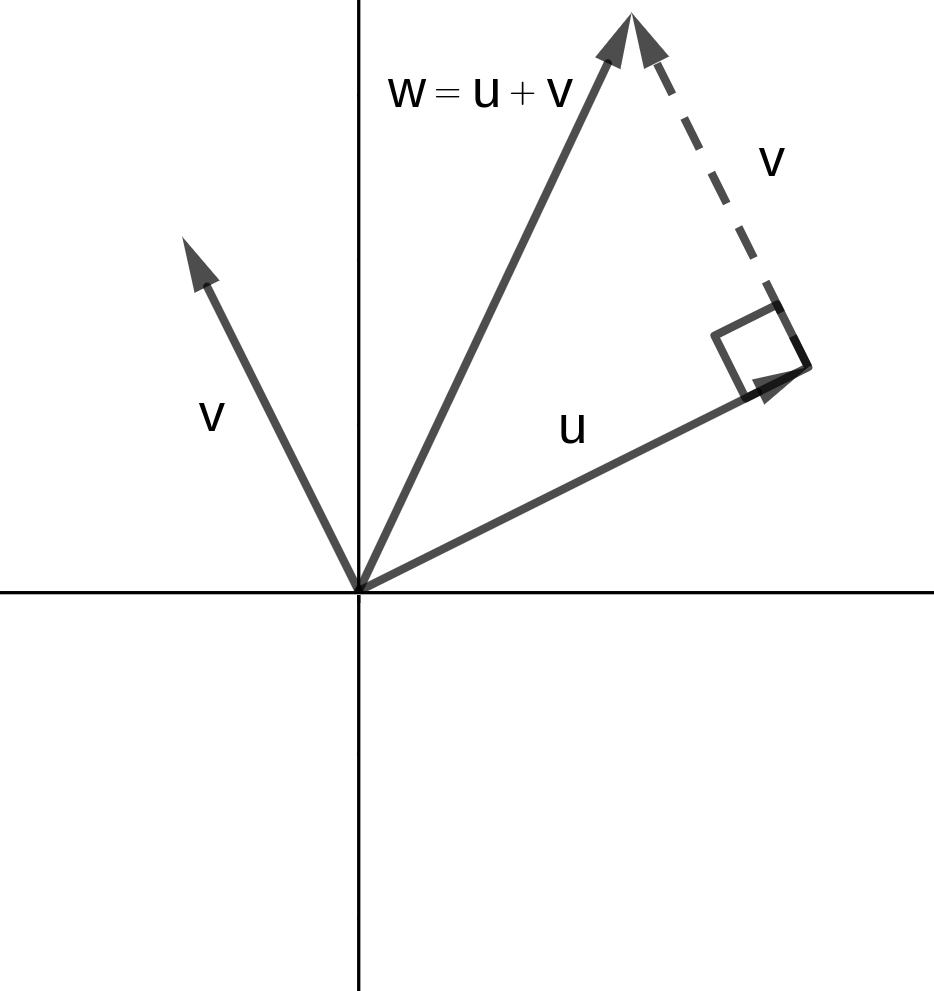
\includegraphics[scale=0.8]{apuntes_algebra_lineal_01.png}
\end{center}
Por el momento, para encontrar una caracteristica que sea equivalente al teorema de Pit\'agoras, vamos a usar a $\overline{w} = \overline{u}+ \overline{v}$, pero es f\'acil convencerse de que la demostraci\'on es v\'alida para cualquier caso. Entonces, se tiene que:
\begin{eqnarray*}
 \lVert \overline{u} \rVert^2 + \lVert \overline{v} \rVert^2 = \lVert \overline{w} \rVert^2 & \Leftrightarrow & \lVert \overline{u} \rVert^2 + \lVert \overline{v} \rVert^2 = \lVert \overline{u} + \overline{v} \rVert^2 \\ 
  & \Leftrightarrow & \overline{u}\cdot \overline{u} + \overline{v}\cdot \overline{v} = \left( \overline{u} + \overline{v} \right)\cdot\left( \overline{u} + \overline{v} \right) \\
  & \Leftrightarrow & \cancel{\overline{u}\cdot \overline{u}} + \cancel{\overline{v}\cdot \overline{v}} = 
  \cancel{\overline{u}\cdot \overline{u}} + \overline{u}\cdot \overline{v}+ \overline{v}\cdot \overline{u} + \cancel{\overline{v} \cdot\overline{v}} \\
  & \Leftrightarrow & \overline{u}\cdot \overline{v} + \overline{\overline{u}\cdot \overline{v}} = 0 \\
  & \Leftrightarrow & 2Re\left( \overline{u}\cdot \overline{v} \right) = 0 \\ 
  & \Leftrightarrow & Re\left( \overline{u}\cdot \overline{v} \right) = 0
\end{eqnarray*}
De aqu\'{\i} que es claro que en un espacio euclideo, es equivalente el Teorema de Pit\'agoras con la definici\'on de ortogonalidad que conocemos: que dos vectores, $\overline{u}$ y $\overline{v}$, son ortogonales si $\overline{u}\cdot \overline{v} = 0$.
\par 
¿Pero qu\'e pasa con los espacios unitarios? ¿No deber\'{\i}a ser equivalente nuestra idea del teorema de Pit\'agoras, con la definici\'on usual de ortogonalidad? Bueno, lo que ocurre es que la construcci\'on fue hecha con base a un teorema ``d\'ebil'' de Pit\'agoras en espacios normados. Pero la definici\'on usual de vectores ortogonales s\'{\i} que es equivalente si modificamos el pitagoras levemente. Esto es:
\begin{teorema}
 Para cualesquiera dos vectores, $\overline{v}$ y $\overline{w}$, en un espacio producto interno complejo son equivalentes las siguientes afirmaciones:
 \begin{itemize}
  \item $\lVert \alpha \overline{v} \rVert^2 + \lVert \beta \overline{w} \rVert^2 = \lVert \alpha \overline{v} + \beta\overline{w} \rVert^2$, para cualesquiera $\alpha$ y $\beta$ escalares.
  \item $\overline{v} \cdot \overline{w} = 0$
 \end{itemize}
\end{teorema}

\begin{demostracion}
 Se deja al lector.
\end{demostracion}

Por lo tanto, decir que dos vectores formar\'an un \'angulo recto si cumplen el teorema de Pit\'agoras es equivalente a decir que estos dos vectores forman un \'angulo recto, o que son ortogonales, si su producto punto es igual a 0, lo cual conviene m\'as para las cuentas que siguen. Por lo tanto podemos crear una definici\'on como sigue para la ortogonalidad:

\begin{definicion}
 Sea $V$ un espacio producto interno. Se dice que $\overline{v},\overline{w}\in V$ son \textit{vectores ortogonales} si $\overline{v}\cdot\overline{w}=0$.\footnote{En muchos libros, cuando esto ocurre, se suele escribir $\overline{v}\perp\overline{w}$.}
\end{definicion}

\begin{observaciones}
 El vector $\overline{o}$ es ortogonal a cualquier vector.
\end{observaciones}


\subsection{Proyecci\'on ortogonal}

Ahora que se ha caracterizado al \'angulo recto y que podemos hablar de vectores ortogonales, se desea conocer qu\'e significar\'{\i}a un \'angulo cualquiera entre dos vectores. Para esto vamos a usar un par de vectores que no sean ortogonales (como el vector nulo es ortogonal a cualquier vector, vamos a pedir que ninguno de los dos vectores sea nulo).
\par 
Para lograr nuestro cometido, vamos a requerir la ayuda de lo que se conoce como \textit{proyecci\'on ortogonal del vector $\overline{v}$ a lo largo del vector $\overline{u}$}, esto es: encontrar un vector en el subespacio generado por $\overline{u}$, $c\overline{u}$, tal que exista un vector $\overline{w} \in V$ que cumpla que $c\overline{u} + \overline{w} = \overline{v}$ y que $\overline{w}\cdot \left( c\overline{u} \right) = 0$. La primera condici\'on nos indica, en un sentido geom\'etrico, que a trav\'es de $\overline{w}$, se puede llegar de $c\overline{u}$ a $\overline{v}$, o lo que es lo mismo $c\overline{u}$, $\overline{v}$ y $\overline{w}$ forman un tri\'angulo; la segunda condici\'on nos indica que $c\overline{u}$ y $\overline{w}$ son ortogonales. Es decir, la interpretaci\'on geom\'etrica de la proyecci\'on ortogonal, que se puede ver en la figura siguiente, es formar con los tres vectores ya mencionados un tri\'angulo rect\'angulo. \begin{center}
 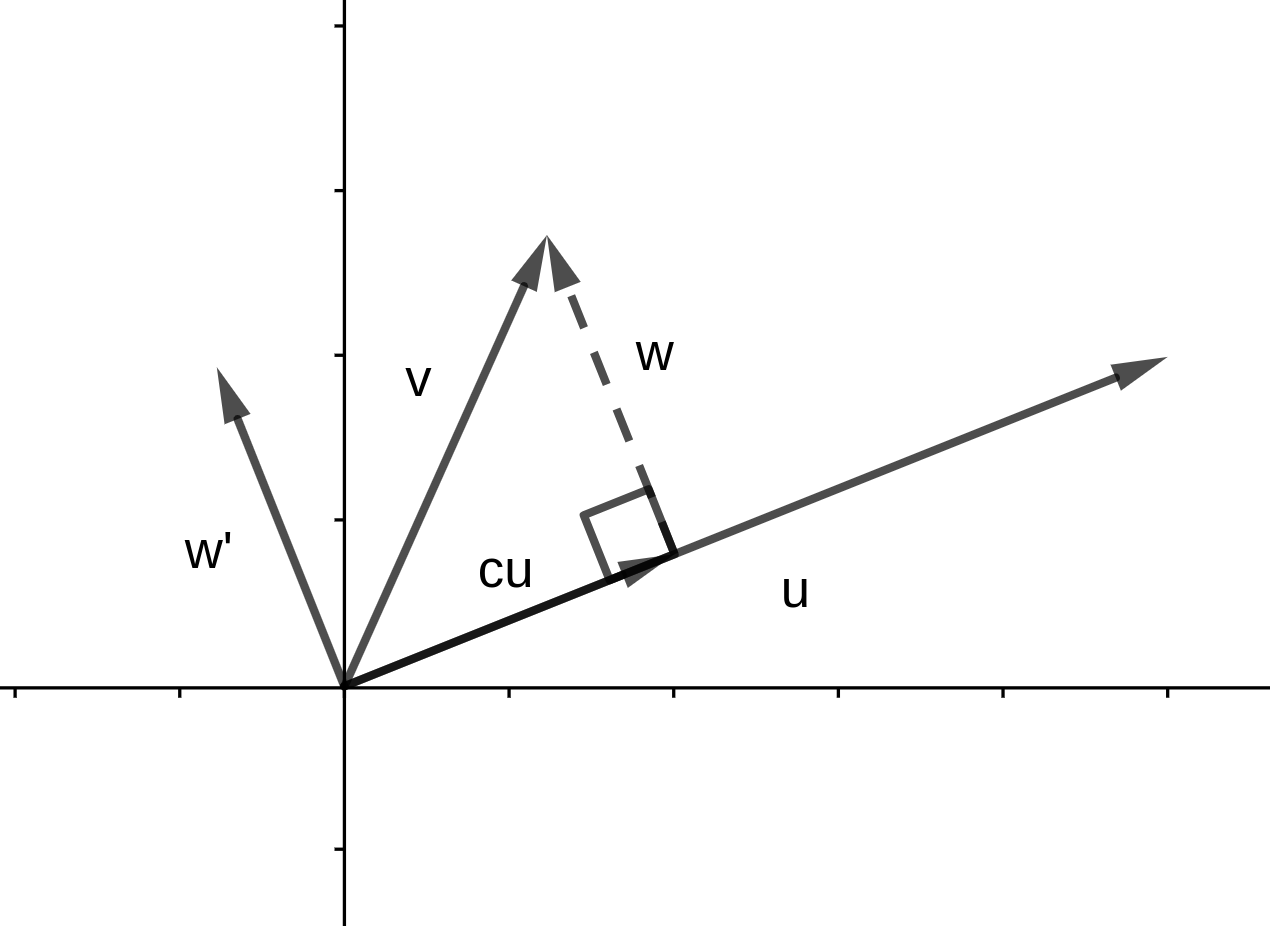
\includegraphics[scale=0.8]{apuntes_algebra_lineal_02.png}
\end{center}
Con ayuda de esto y un poco de trigonometr\'{\i}a podremos definir un \'angulo entre vectores, ya que, si llamamos $\theta$ al \'angulo entre $c\overline{u}$ y $\overline{v}$, podemos definir el coseno de $\theta$ como:
\begin{equation}
 \cos \theta = \frac{\lVert c\overline{u} \rVert}{\lVert \overline{v} \rVert}
\end{equation}
y de ah\'{\i} obtener el \'angulo como el coseno inverso del cociente.
\begin{teorema}
 Sean $\overline{u}$ y $\overline{v}$ vectores no nulos y no ortogonales en el espacio producto interno $V$, entonces existe un \'unico vector, $c\overline{u} \neq \overline{o}$, en el subespacio generado por $\overline{u}$ tal que existe un vector $\overline{w} \in V$ que cumple que $c\overline{u} + \overline{w} = \overline{v}$ y que $\overline{w}\cdot \left( c\overline{u} \right)=0$, y \'este, est\'a definido por el escalar
 \begin{equation}
  c = \frac{\overline{v}\cdot \overline{u}}{\lVert \overline{u} \rVert^2}
 \end{equation}
\end{teorema}
\begin{demostracion}
 si $c\overline{u} + \overline{w} = \overline{v}$, entonces
 \begin{equation}
  \overline{w} = \overline{v} - c\overline{u}.
 \end{equation}
 Por lo tanto, y usando que $c\overline{u} \neq \overline{o}$ implica que $c \neq 0$, se obtienen las siguientes equivalencias.
 \begin{eqnarray*}
  \overline{w}\cdot \left( c\overline{u} \right) = 0
   & \Leftrightarrow & \left( \overline{v} - c\overline{u} \right)\cdot \left( c\overline{u} \right) = 0 \\ 
   & \Leftrightarrow & \overline{v}\cdot \left( c\overline{u} \right) - \left( c\overline{u} \right) \cdot \left( c\overline{u} \right) = 0 \\
   & \Leftrightarrow & \overline{c} \left( \overline{v} \cdot \overline{u} \right) - \lVert c\overline{u} \rVert^2 = 0 \\
   & \Leftrightarrow & \lvert c \rvert^2 \lVert \overline{u} \rVert^2 = \overline{c} \left( \overline{v} \cdot \overline{u} \right) \\
   & \Leftrightarrow & \frac{\lvert c \rvert^2}{\overline{c}} = \frac{\overline{v} \cdot \overline{u} }{\lVert \overline{u} \rVert^2} 
 \end{eqnarray*}
 Por lo tanto
 \begin{equation}
  c = \frac{\overline{v}\cdot \overline{u}}{\lVert \overline{u} \rVert^2}
 \end{equation}
 que es a lo que se quer\'{\i}a llegar.${}_{\blacksquare}$
\end{demostracion}

\begin{observaciones}
 Se ha pedido que no sean ortogonales los vectores para poder realizar la divisi\'on entre el conjugado de $c$. En caso de que $c=0$, entonces el vector $c\overline{u} = \overline{o}$ tambi\'en cumplir\'{\i}a lo pedido pero sin aportar nada nuevo. Sin embargo, si los vectores $\overline{u}$ y $\overline{v}$ fuesen ortogonales, entonces llegar\'{\i}amos, usando los mismos pasos, a que $c=0$, ya que
 \begin{eqnarray*}
  \left( \overline{v} - c\overline{u} \right)\cdot \left( c\overline{u} \right) = 0
   & \Leftrightarrow & \overline{c} \left( \overline{v} \cdot \overline{u} \right) - \lVert c\overline{u} \rVert^2 = 0 \\
   & \Leftrightarrow & \lvert c \rvert^2 \lVert \overline{u} \rVert^2 = \overline{c} \left( \overline{v} \cdot \overline{u} \right) \\
   & \Leftrightarrow & \lvert c \rvert^2 \lVert \overline{u} \rVert^2 = 0 \\
   & \Leftrightarrow & \lvert c \rvert^2 = 0 \\
   & \Leftrightarrow & c = 0
 \end{eqnarray*}
 lo cual tambi\'en se aplica para la f\'ormula dada.
\end{observaciones}
La observaci\'on anterior nos permite entonces definir, de manera ya general, lo siguiente:
\begin{definicion}
 Sean $\overline{v}$ y $\overline{w}$ vectores no nulos en el espacio producto interno $V$, entonces definimos al vector $c\overline{w}$ como la\textit{proyecci\'on ortogonal de $\overline{v}$ a lo largo de $\overline{w}$}, si $c$ es el escalar
 \begin{equation}
  c = \frac{\overline{v} \cdot \overline{w}}{\overline{w}\cdot\overline{w}} = \frac{\overline{v} \cdot \overline{w}}{\lVert \overline{w} \rVert^2}
 \end{equation}
 y se define $c$ como la \textit{componente} de $\overline{v}$ a lo largo de $\overline{w}$.
\end{definicion}

\subsection{Ahora s\'{\i}: el coseno del \'angulo de dos vectores}

Como se mencion\'o antes, la interpretaci\'on geom\'etrica de la proyecci\'on ortogonal de $\overline{v}$ sobre $\overline{w}$ de un vector sobre otro, nos permite construir un tri\'angulo rect\'angulo, en donde $c\overline{w}$ representa el cateto adyacente al \'angulo $\theta$ y $\overline{v}$ representa la hipotenusa. En tal caso, y de forma general, podemos entonces definir el coseno del \'angulo $\theta$ entre estos dos vectores como el cociente de sus longitudes. esto es:
\begin{equation}
 \cos \theta = \frac{\lVert c\overline{w} \rVert }{\lVert \overline{v} \rVert} 
 = \frac{ \left\lvert \frac{\overline{v}\cdot \overline{w}}{ \lVert \overline{w} \rVert^{\cancel{2}}} \right\rvert \cancel{\lVert\overline{w}\rVert}}{\lVert \overline{v} \rVert} 
 = \frac{\lvert \overline{v}\cdot \overline{w} \rvert}{\lVert \overline{v} \rVert \lVert \overline{w} \rVert}
\end{equation}
que, por la desigualdad de Schwartz, se sabe que
\begin{equation*}
 \frac{\lvert \overline{v} \cdot \overline{w} \rvert}{\lVert \overline{v} \rVert \lVert \overline{w} \rVert} \leq 1
\end{equation*}
por lo que tiene sentido definir de este modo el coseno del \'angulo.
\par 
Es notable observar que en esta definici\'on, el coseno del \'angulo s\'olo puede vivir entre los valores $0$ y $1$, esto quiere decir que para esta definici\'on, se tiene que restringir el \'angulo entre vectores donde el coseno no sea negativo. Para nuestra construcci\'on, lo podemos restringir a \'angulos desde $0^{\circ}$ a $90^{\circ}$.
\par 
Por otro lado, esta construcci\'on se ha hecho para obtener el coseno del \'angulo entre $\overline{v}$ y $c\overline{w}$. Si denotamos como $ang\left(\overline{v}, \overline{w}\right)$ al \'angulo entre los vectores $\overline{v}$ y $\overline{w}$, como el \'angulo que hemos definido es un valor entre los $0^{\circ}$ y los $90^{\circ}$ deber\'{\i}amos obtener el mismo \'angulo para cualesquiera segmentos sobre la rectas que definen ese \'angulo. Esto se traduce en espacios vectoriales diciendo que, si est\'a bien definido el \'angulo como se ha hecho, deber\'{\i}a ocurrir que $ang(\overline{v}, \overline{w}) = ang(\overline{v}', \overline{w}')$ para cualesquiera vectores no nulos $\overline{v}'$ en el espacio generado por $\overline{v}$ y $\overline{w}'$ en el espacio generado por $\overline{w}$.
\par 
Con lo anterior, vamos entonces a definir el coseno del \'angulo entre $\overline{v}$ y $\overline{w}$ como se ha hecho con el coseno del \'angulo entre $\overline{v}$ y $c\overline{w}$, es decir:
\begin{equation*}
 \cos \left( ang\left( \overline{v}, \overline{w} \right) \right) = \frac{\lvert \overline{v} \cdot \overline{w} \rvert}{\lVert \overline{v} \rVert \lVert \overline{w} \rVert}
\end{equation*}
Entonces, si $\lambda \neq 0$ es un escalar cualquiera, $\lambda \overline{w}$ es un vector no nulo en el subespacio generado por $\overline{w}$, entonces:
\begin{equation}
 \cos\left( ang\left( \overline{v}, \lambda \overline{w} \right) \right) =
 \frac{\lvert \overline{v}\cdot \left( \lambda \overline{w} \right) \rvert}{\lVert \overline{v} \rVert \lVert \lambda \overline{w} \rVert} =
 \frac{\lvert \overline{\lambda} \left( \overline{v} \cdot \overline{w} \right) \rvert}{\lvert \lambda \rvert \lVert \overline{v} \rVert \lVert \overline{w} \rVert} =
 \cancelto{1}{\frac{\lvert \overline{\lambda} \rvert}{\lvert \lambda \rvert}} \frac{\lvert \overline{v} \cdot \overline{w} \rvert}{\lVert \overline{v} \rVert \lVert \overline{w} \rVert} = \cos\left( ang\left( \overline{v},\overline{w} \right) \right)
\end{equation}
An\'alogamente, es f\'acil comprobar que para $\lambda \neq 0$ se cumple que $\cos\left(ang\left( \lambda\overline{v},\overline{w} \right)\right) = \cos\left( ang\left( \overline{v}, \overline{w} \right) \right)$.
\par 
Ya con esto, concluimos lo siguiente:
\begin{definicion}
 Sea $\overline{v}$ y $\overline{w}$ dos vectores no nulos de un espacio producto interno $V$.
 El \'angulo que forma el vector $\overline{v}\neq\overline{o}$ con el vector $\overline{w}\neq \overline{o}$, que se denota poniendo $\text{\'ang}\left( \overline{v},\overline{w}\right)$ \'o $\widehat{\left( \overline{v}, \overline{w} \right)}$, queda caracterizado por su coseno, que vale:
 \begin{equation}
  \cos(\overline{v}, \overline{w}) = \frac{\lvert \overline{v}\cdot \overline{w} \rvert}{\lVert \overline{v} \rVert \lVert \overline{w} \rVert}
 \end{equation}
 La medida del \'angulo queda definido en el rango $\text{\'ang}\left( \overline{v},\overline{w}\right) \in \left[0, \frac{\pi}{2}\right]$.
\end{definicion}

\begin{observaciones}
 Ya para acabar un par de observaciones:
 \begin{itemize}
  \item La definici\'on que se ha dado, ha sido para espacios vectoriales generales. Tenga en cuenta que cuando el espacio es euclideo, entonces tiene sentido hablar de escalares positivos y negativos, por lo que el \'angulo se puede mover extender para cosenos negativos. En tal caso, es cuando queda definido como
  \begin{equation}
   \cos\left( \overline{v}, \overline{w} \right) = \frac{\overline{v} \cdot \overline{w}}{\lVert \overline{v} \rVert \lVert \overline{w} \rVert};
  \end{equation}
  sin embargo, si habl\'aramos, por ejemplo, de escalares complejos, entonces el coseno podr\'{\i}a tomar valores complejos, por lo que habr\'{\i}a que hacer un an\'alisis m\'as detallado... Y la verdad es que hasta aqu\'{\i} llego. Ya me convenc\'{\i} de la f\'ormmula. De cualquier forma, s\'{\i} me puse a investigar qu\'e ser\'{\i}a un \'angulo sobre un espacio unitario, pero siempre se define sobre espacios euclideos, por lo que supongo que tiene poca importancia y no creo que valga la pena gastar m\'as tiempo en investigar eso. Si alguien que lee estas nota sabe, agradecer\'{\i}a mucho que me dijera.
  \item En efecto, el libro que me hizo construir todo esto no toca varias definiciones hasta el momento de tomar el tema del \'angulo, por lo que tiene sentido no haberlo construido de este modo. De todas formas, sigue habiendo un pendiente: seg\'un el libro, se menciona que el dichoso ap\'endice 11 (que no aparece en el libro) define el \'angulo con precisi\'on usando rotaciones en el plano. Me queda entonces el pendiente de c\'omo Juan de Burgos construye entonces esa definici\'on, pero al menos eso en lo personal ya no me interesa tanto, pues he construido aqu\'{\i} la definici\'on de modo que tenga sentido. As\'{\i}, pues, yo ya estoy satisfecho, y espero que el lector tambi\'en.
 \end{itemize}

\end{observaciones}



\end{document}
